\section{Theorie}
\label{sec:Theorie}
\subsection{Zielsetzung}
Ziel des Versuchs ist die Überprüfung der Bragg-Bedingung, die Messung des Emissionspektrum für einer Cu-Anode
einer Röntgenröhre und die Bestimmung der Abschirmungskonstanten $\sigma_K$ für verschiedene Materialien durch Messung ihrer Absorptionsspektren.
\subsection{Erzeugung von Röntgenstrahlung}
Röntgenstrahlen können durch die Abbremsung schneller Elektronen erzeugt werden. Dafür wird in einer Röntgenröhre an einer
Glühkathode Elektronen emittiert, die mit einer Spannung im kV Bereich zur Anode hin beschleunigt werden. Beim Auftreffen auf das Anodenmaterial werden 
die Elektronen im Coulombfeld der Atomkerne abgebremst. Die Differenz der kinetischen Energie wird als Photon abgestrahlt. Dieser Teil des Spektrums wird als kontinuierliches 
Bremsspektrum bezeichnet, da jeder beliebige Teil der kinetischen Energie abgegeben werden kann. Der Anteil ist in Abbildung \ref{fig:Brems} zu sehen.
\begin{figure}[H]
    \centering
    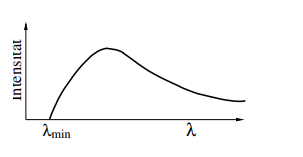
\includegraphics[scale=1.5]{content/Bremsspektrum.png}
    \caption{Bremsspektrum der Röntgenstrahlung \cite{sample}.}
    \label{fig:Brems}
\end{figure}
\noindent Die maximale Energie der Photonen kann anhand der minimalen Wellenlänge$\lambda_\text{min}$ abgelesen werden. Diese ergibt sich aus der angelegten Spannung $U$
durch die Formel
\begin{equation}
    \lambda_\text{min}=\frac{h\cdot c}{e_0U}.
    \label{eq:minWelle}
\end{equation}
und beschreibt die Elektronen, die vollständig abgebremst worden sind und somit ihre gesamte kinetische Energie $E_\text{kin}=e_0U$ als Photon mit Energie $E=h\nu$ abgegeben haben.
Zusätzlich existiert noch ein für das Anodenmaterial charakteristisches Spektrum. Es entsteht, da die Elektronen das Anodenmaterial ionisieren und dadurch
Elektronen in die innere Schale zurückfallen können. Die Energiedifferenz $E_m-E_n$ der Schalen wird als Photon emittiert und ist Teil des Röntgenspektrums.
Kontinuierliches und charakteristisches Spektrum überlagern sich gemeinsam zum gemessenen Röntgenspektrum
\subsection{Emissionspektrum}
Das Emissionspektrum besteht aus scharfen Linien, die durch die diskreten
Energieübergänge im Anodenmaterial quantisiert sind. Die Linien können dadurch charakterisiert werden
indem die Schalen n=1,2,3 in die Elektronen fallen mit K,L,M... bezeichnet werden und die Schale aus der die Elektronen kommen
mit aufsteigenden griechischen Buchstaben bezeichnet werden. $K_\alpha$ bezeichnet dann einen Übergang aus der L in die K-Schale, $K_\beta$ einen Übergang
vom M in die K Schale und $L_\alpha$ den Übergang aus der M in die L Schale. Die Energie einer Schale ist charakterisiert durch einen Anteil der Rydbergenergie $R_\infty=\qty{13.6}{\eV}$, der 
Grundzustandsenergie des Wasserstoffatoms. Dabei ist bei Mehrelektronensytemen zu beachten, dass die Kernladung durch die Hüllenelektronen
abgeschirmt wird, sodass eine effektive Kernladung $z_\text{eff}=z-\sigma$ mit Abschirmungskonstante $\sigma$ eingeführt werden muss.
Damit ergibt sich allgemein für die Bindungsenergie
\begin{equation}
    E_n = -R_\infty z_\text{eff}^2\cdot \frac{1}{n^2}
    \label{eq:En-Emission}
\end{equation}
und für die Energie der einzelnen Linien
\begin{equation}
    \Delta E =E_m-E_n= R_\infty ((z-\sigma_n)^2\cdot \frac{1}{n^2}-(z-\sigma_m)^2\cdot \frac{1}{m^2}).
    \label{eq:dE-Emission}
\end{equation}
Die Absorptionskonstante ist materialabhängig uns kann empirisch bestimmt werden.
Im Allgemeinen sind sie charakteristischen Linien nicht beliebig scharf, sondern sind in Wahrheit eine Überlagerung einzelner sehr dicht nebeneinander liegender Linien.
Dies liegt daran, dass einzelnen Elektronen einer Schale je nach
Bahndrehimpuls und Elektronenspin eine leicht unterschiedliche Energie besitzen. Diese Aufspaltung wird Feinstruktur genannt.
\subsection{Absorptionsspektrum}
Die Absorption von Röntgenstrahlung läuft vom Prinzip sehr ähnlich zur Emission ab. Photonen 
mit einer Energie größer der Bindungsenergie der Elektronen einer Schale können das Atom unter Aufnahme des Photons vollständig
absorbieren. Generell werden können energiereichere Photonen schlechter absorbiert werden. Nur das Überschreiten gewisser Bindungsenergien
erhöht die Absorptionshäufigkeit. Dadurch ergeben sich bei den einzelnen Energien der Schalen charakteristische Kanten, die wie bei
der Emission K,L,M... Absorptionskante genannt werden. Eine schematische Darstellung ist in 
Abbildung \ref{fig:Absorption} zu sehen.
\begin{figure}[H]
    \centering
    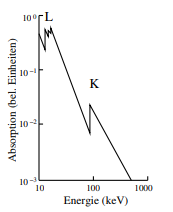
\includegraphics[scale=1.5]{content/Absorption.png}
    \caption{Absorptionskanten\cite{sample}.}
    \label{fig:Absorption}
\end{figure}

\noindent Um die Absorptionskonstante allgemein zu bestimmen muss die Sommerfeldsche Feinstrukturformel
\begin{equation}
    E_{nj}=-R_\infty \left(z_\text{eff}^2\cdot \frac{1}{n^2}+\alpha^2z_\text{eff}^4\cdot \frac{1}{n^3}\cdot\left(\frac{1}{j+\frac{1}{2}}-\frac{3}{4n}\right)\right)
    \label{eq:Sommerfeld}
\end{equation}
benutzt werden. Dabei beschreibt $n$ die Hauptquantenzahl und $l$ der Gesamtdrehimpuls des betrachteten Elektrons und $\alpha$ die Sommerfeldsche Feinstrukturkonstante.
Für Elektronen aus der K-Schale ist $n=1$ und $j=0$ ergibt sich die Abschirmungskonstante zu 
\begin{equation}
    \sigma_K=Z-\sqrt{\frac{E_K}{R_\infty}-\frac{\alpha^2Z^4}{4}}.
    \label{eq:Abschirm}
\end{equation} 
$E_K$ beschreibt die Energie der K-Kante.
\subsection{Bragg-Bedingung}
Die Beugung von Photonen an einem dreidimensionalem Kristallgitter wird Bragg'sche Reflexion genannt.
Die Interferenz der Photonen bewirkt, dass ein Interferenzmaximum beim doppelten Drehwinkel des Kristalls, dem sogenannten Glanzwinkel $\Theta$, beobachtet werden kann.
Die Beugung ist in Abbildung \ref{fig:Bragg} abgebildet.
Die Bragg Bedingung ausgeschrieben lautet
\begin{equation}
    2d \sin\theta=n\lambda.
\end{equation}
\begin{figure}[H]
    \centering
    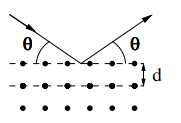
\includegraphics[scale=1.5]{content/Bragg.png}
    \caption{Bragg'sche Reflexion\cite{sample}.}
    \label{fig:Bragg}
\end{figure}

\cite{sample}
